% !TeX root = OptCuts.tex

\section{Evaluation}
\label{sec:results}

\subsection{Implementation}

\danny{Minchen - I added this subsection. Please put here all pertinant details about the implementation that are not core contributions - e.g. the initialization subsection I moved below; the details on your smooth iteration step I also moved below; your missing details about bijectviity that you mention below. Also put here any important details of the libraries you used and the and specs of the machine(s) used to time and evaluate methods, etc.}

\minchen{Text possibly needed in the description of how we handle global bijectivity:
When computing $\hat{f}_e$, besides also including the one-ring triangles on the scaffold mesh for computing energy decrease, we also need to move the splitted vertices slightly apart to leave room for inserting new scaffold mesh triangles.}

\subsubsection{Initialization}
To obtain an initial UV map for an input surface, we map its initial seam to a circle preserving edge length and parameterize the rest of the vertices through Tutte embedding with uniform weights.

We compute initial seams for different surfaces according to their topology and geometry. For disk-topology surfaces, we simply pick their longest boundary as the initial seam. For genus-0 closed surfaces, we randomly pick 2 connected edges as the initial seam. \minchen{[TODO] change to curvest one point cut or farthest point cut if they are better} For high-genus surfaces, we follow Crane et al.~\shortcite{Crane:2013:DGP} to detect homology generators and connect all of them as the initial seam \minchen{[TODO]}.

We simply start by ignoring the distortion constraints with $\lambda$ set to $0$, and let our dual update to modify $\lambda$ according to the intermediate distortions.

\subsubsection{Continuous Search}
\label{sec:descentStep}

Our smooth descent steps take in the locally altered UV map by the current topology descent step and conduct one Newton-type iteration towards solving $\min_U E_d$ with $T$ fixed (Algorithm~\ref{alg:descentStep}).

\begin{algorithm}[h]
\SetAlgoLined
\KwData{$M$, $T^{k,i}$, $U_a^{k,i-1}$}
\KwResult{$U^{k,i}$, $\delta^{k,i}$}
$g^{k,i-1} \leftarrow \nabla E_{SD}(T^{k,i}, U_a^{k,i-1})$\;
\If{$||g^{k,i-1}||^2 < 10^{-8}$}{
	converge\;
}
compute $E_{SD}$ Hessian proxy $P^{k,i-1}$\;
solve $P^{k,i-1} p^{k,i-1} = -g^{k,i-1}$ for search direction $p^{k,i-1}$\;
compute initial step size $\alpha^{k,i-1}_0$\;
back-tracking line search with Armijo rule to obtain $\alpha^{k,i-1}$\;
$U^{k,i} \leftarrow U_a^{k,i-1} + \alpha^{k,i-1} p^{k,i-1}$\;
$\delta^{k,i} \leftarrow E_{SD}(T^{k,i}, U^{k,i}) - E_{SD}(T^{k,i}, U_a^{k,i-1})$\;
\If{$|\delta^{k,i}/E_{SD}(T^{k,i}, U_a^{k,i-1})| < 10^{-6}\alpha^{k,i-1}$}{
	stop\;
}
\caption{Smooth Descent Step $(k+1,i)$}
\label{alg:descentStep}
\end{algorithm}
Since $E_{SD}$ is not convex, we apply the projected Newton method~\cite{Teran2005Robust} to project the Hessian of each energy element to its closest symmetric positive definite (SPD) matrix in parallel, and assemble them to form the SPD Hessian proxy $P$. We use the PARDISO~\cite{pardiso-6.0a, pardiso-6.0b} symmetric indefinite solver to solve the linear system $P p = -g$ for search direction $p$. \justin{personally I'd move mention of pardiso to implementation section}\minchen{[TODO] change to use SPD solver by fixing a direction to ensure definiteness} As $E_{SD}$ is also a barrier-type energy, it is essential to ensure that the configuration always stays inside the feasible region. Thus, we follow Smith and Schaefer~\shortcite{Smith2015Bijective} to first compute an initial step size $\alpha_0$ that avoids element inversion and then conduct back-tracking line search with Armijo rule~\cite{Armijo1966Minimization} to ensure sufficient energy decrease.

Besides a relatively small tolerance on $g$ for convergence detection, we apply another relative energy decrease criteria to appropriately stop the process while necessary.
This can stop our continuous search at the true local optimum infinitesimal better than setting a larger gradient tolerance since our energy is highly nonlinear.

\vova{Explain how to handle bijectivity...}

%\paragraph{Potential Accelerations for Practical Use}
%Since our topological operations only change the mesh locally both on connectivity and coordinates, we could also update the Hessian or the decomposition locally to save time. Besides, it is also interesting to try other Hessian approximation methods like L-BFGS~\cite{Liu1989Limited} or composite majorization~\cite{Shtengel2017Geometric} to explore further acceleration by finding a balance between per-iteration computational cost and convergence rate.
%\justin{not sure previous paragraph is needed}

\subsection{Method Evaluation}

We evaluate our method with/without global bijectivity by running them on 70 input surfaces, including both disk-topology and closed surfaces, some are with \minchen{[TODO] high genus}, setting $b_d$ to $4.2$, $4.1$, and $4.05$ (Figure~\ref{fig:our_impressive_results}).

\begin{figure}[!h]
\centering
% \includegraphics[width=\linewidth]{fig/our_impressive_results.png}
\caption{UV maps generated by our methods with/without bijectivity given $b_d = 4.2, 4.1, 4.05$.}
\label{fig:our_impressive_results}
\end{figure}

\paragraph{Evaluation Metric}
We are able to directly use the output normalized $E_{SL}$ as the evaluation metric since our method can generate UV maps with locally optimal seams under a certain distortion bound. This metric can be consistent among comparisons against all methods because given an input surface we are always able to compare the output $E_{SL}$ under the same level of distortion. Moreover, it also fits in well with practical scenarios where the control of distortions are more intuitive to the users and as-short-as-possible seams are expected.

\paragraph{Initial Embedding}
\minchen{[do we want this?]} To show that we search for locally optimal UV maps regardless of the given initial embedding, we run our method starting from our standard initializations, triangle soups, and preliminary UV maps produced by other methods or by users. As demonstrated in Figure~\ref{fig:bad_init_still_ends_well}, all the output UV maps are with high quality.


\subsection{Comparison}

We demonstrate the capabilities of our framework by comparing to the state-of-the-art AutoCuts~\cite{Poranne2017Autocuts} and the classic seam-cutting method Seamster~\cite{Sheffer2002Seamster}.

\paragraph{AutoCuts}
AutoCuts obtains high quality UV maps by involving users into the optimization loop. However, when aiming for convenient, fully-automatic methods, the non-smoothness of their Separation energy not only makes it challenging for global parameter settings, but also often end up the optimization with suboptimal results. To show that we automatically obtain high quality results without suffering these issues, we compare our method with a fully automatic version of AutoCuts obtained under the guidance of AutoCuts authors by constructing appropriate homotopy paths with a uniform set of mesh-adaptive parameters.

Since AutoCuts does not intuitively support generating UV maps with a certain level of distortion, we first run AutoCuts on a batch of input surfaces, and then set their output distortions as $b_d$ in our method for each input. As demonstrated in Table~\ref{tb:comp_AutoCuts}, for both the two versions of our method, we require less time to generate UV maps with same level of distortion but significantly smaller seams. Figure~\ref{fig:ESLBar_compAutoCuts} shows a bar chart comparison on the output $E_{SL}$ of each input surface. Note that we easily enforced bijectivity (Figure~\ref{fig:comp_AutoCuts}), which is only supported in AutoCuts with user assistance on patch manipulation.

\begin{table}[!h]
\centering
\caption{Comparisons between AutoCuts and our method on 69 input surfaces with $3749$ vertices in average.}
\label{tb:comp_AutoCuts}
\begin{tabular}{|c|ccc|ccc|}
\hline
\multirow{2}{*}{method} & \multicolumn{3}{c|}{$E_{SL}$} & \multicolumn{3}{c|}{time (s)} \\ \cline{2-7} 
                        & avg      & min     & max      & avg      & min    & max       \\ \hline
AutoCuts                & 7.5789   & 1.2069  & 24.6816  & 499.9    & 4.0    & 2677.0    \\
ours (WB)               & 5.8114   & 0.8979  & 19.7405  & 304.0    & 6.4    & 1267.7     \\
ours (NB)               & 5.3065   & 0.8992  & 16.1329  & 148.7    & 3.1    & 650.9    \\ \hline
\end{tabular}
\end{table}

\begin{figure}[!h]
\centering
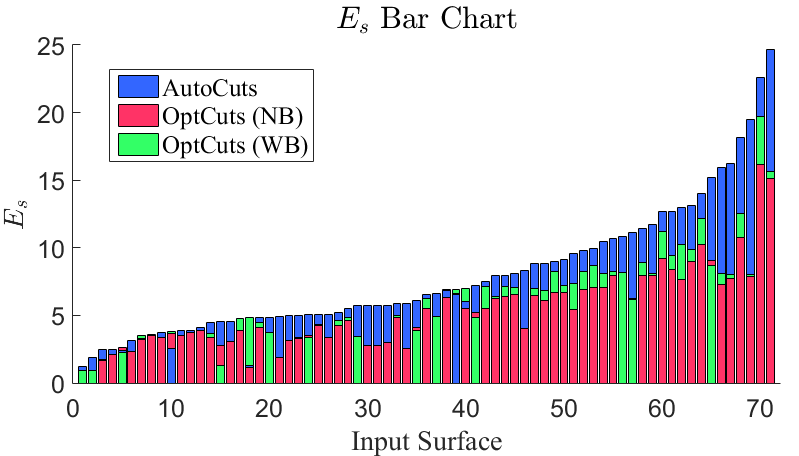
\includegraphics[width=\linewidth]{fig/ESLBar_compAutoCuts.png}
\caption{$E_{SL}$ bar chart of each example generated by AutoCuts and our method with/without bijectivity.}
\label{fig:ESLBar_compAutoCuts}
\end{figure}

\begin{figure}[!h]
\centering
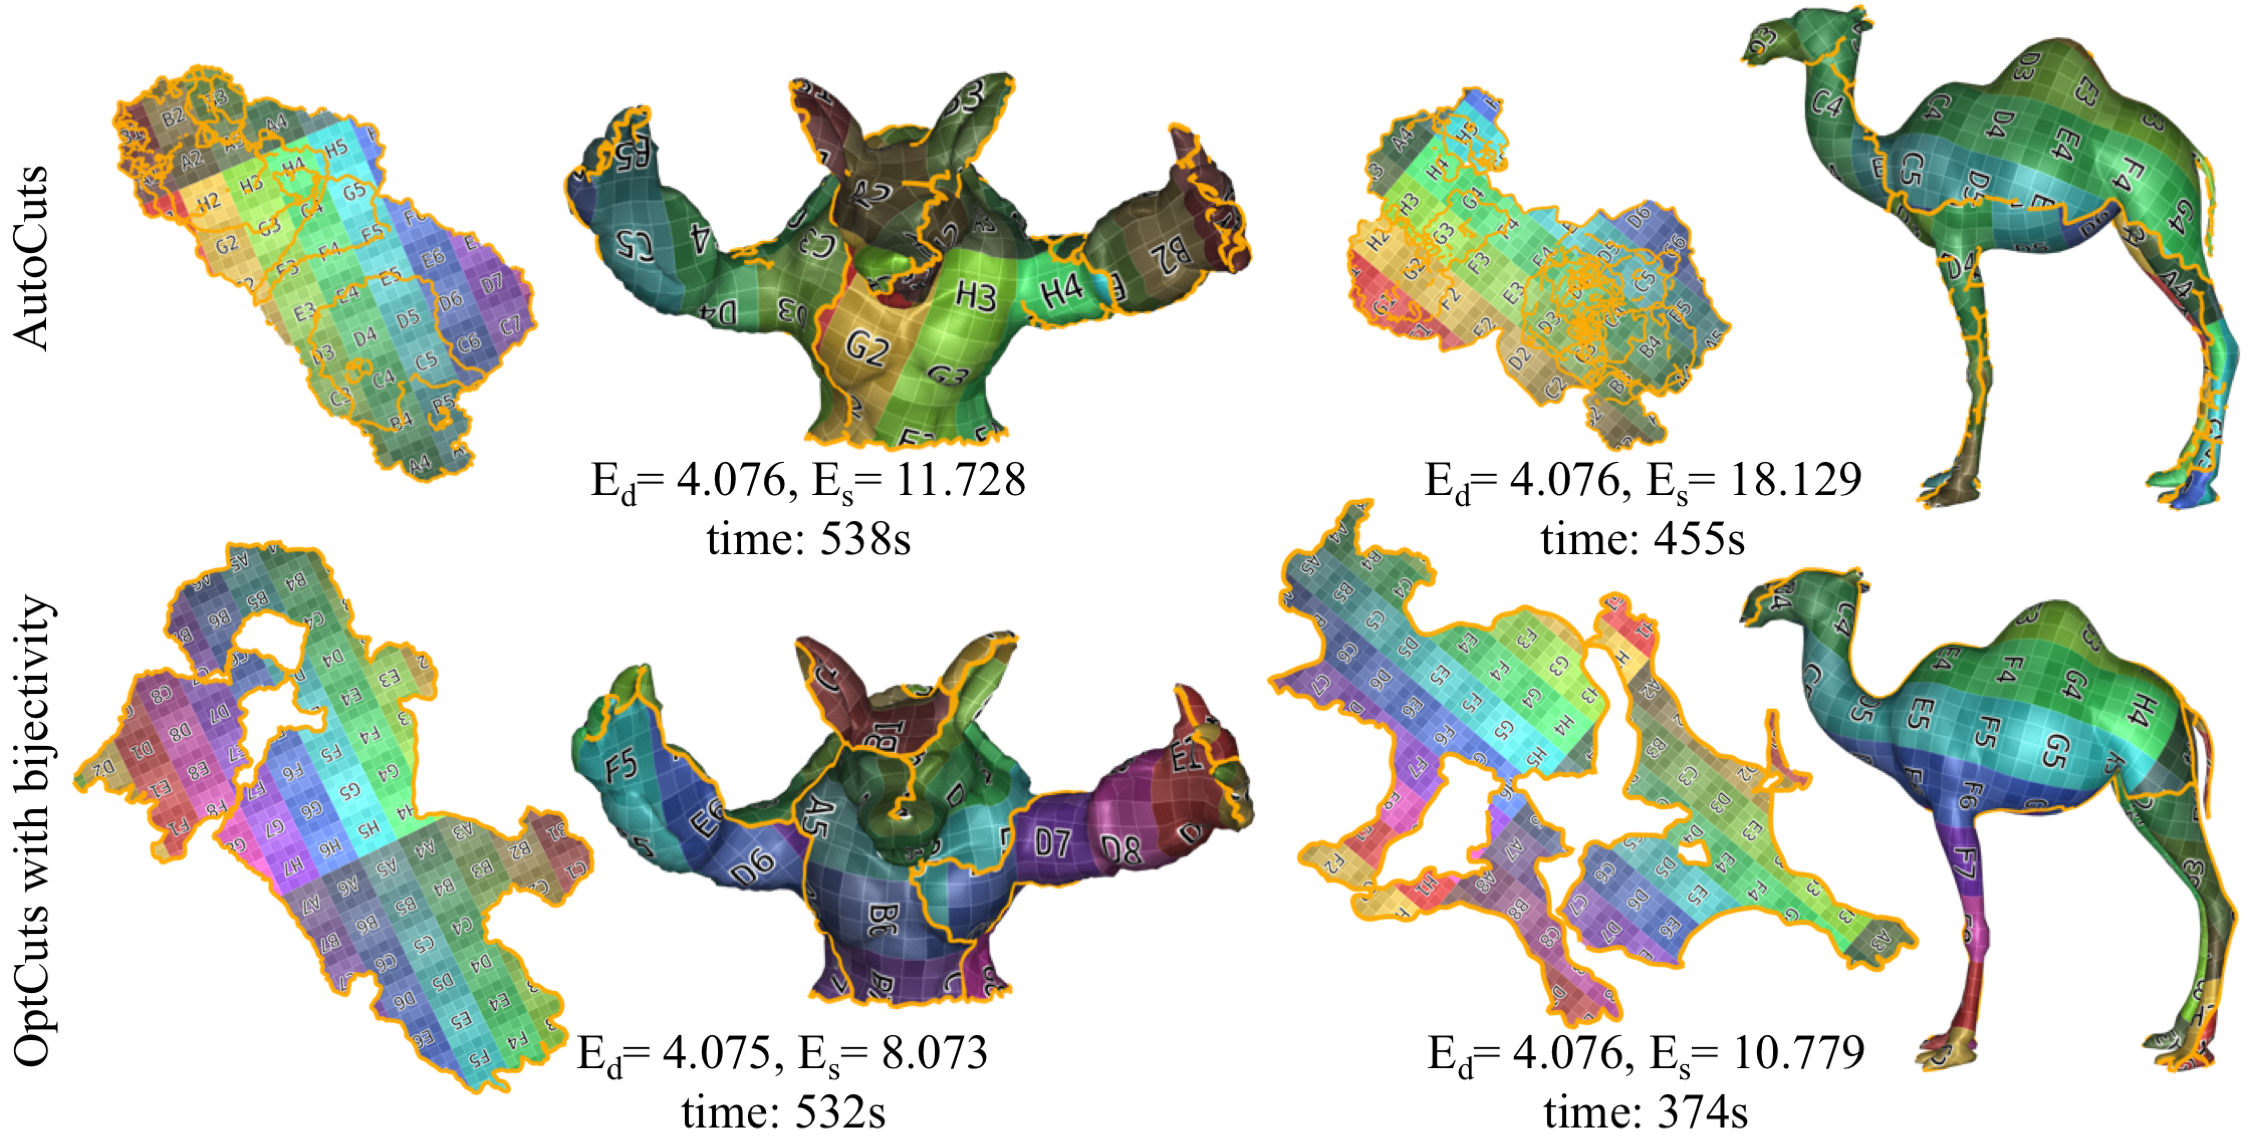
\includegraphics[width=\linewidth]{fig/comp_AutoCuts.png}
\caption{Comparison between AutoCuts and our method on the camel and three man statue model.}
\label{fig:comp_AutoCuts}
\end{figure}
% could also be bone_noInput, bunny_i_f10000, bunny, camel_vova_f10000, cat_noUV, cow_param_closed, dilo, horse, male_2, octopus, wooden_fish, foot_i_f10000, gargoyle, rgb_dragon, statue_i_1, vase, venus

From the time-resolution scatter plot in Figure~\ref{fig:time_res_compAutoCuts}a, we see that for meshes with higher resolution, our method scales better on running time than AutoCuts.
We further run AutoCuts and our methods on 5 input surfaces obtained by progressively simplifying the original lucy model (48354 vertices) to test scalability. From the trend in Figure~\ref{fig:time_res_compAutoCuts}b, we further see that our method scales better. Besides, the average $E_{SL}$ obtained by our methods with/without bijectivity on the lucy models are $9.236$ and $8.816$ respectively, much smaller than $13.052$ by AutoCuts. Notice that for models with 24200 and 48354 vertices, AutoCuts already run out of memory, since its system size is $6$ times that of ours.

\begin{figure}[!h]
\centering
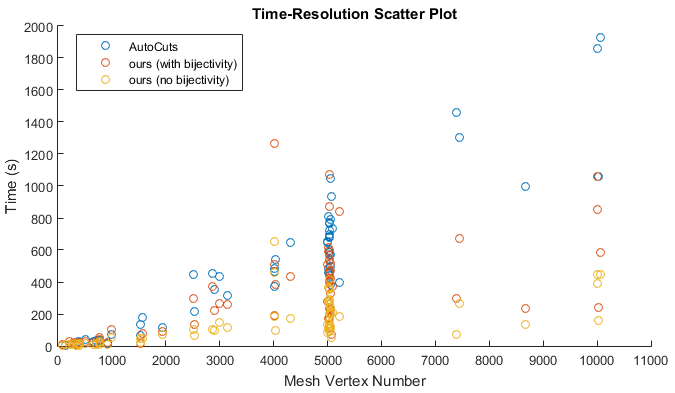
\includegraphics[width=\linewidth]{fig/time_res_compAutoCuts.png}
\caption{Time-resolution scatter plot of a batch of examples (a) and 5 lucy models with different resolutions (b) generated by AutoCuts and our method with/without bijectivity. Note that in (b), there is no data for AutoCuts on models with 24200 and 48354 vertices due to running out of memory.}
\label{fig:time_res_compAutoCuts}
\end{figure}

\paragraph{Seamster}
To compare with Seamster, we first use its output seams on the cow model and the triceraptop model to obtain the UV maps by minimizing $E_{SD}$ with bijectivity constraints, and set the output distortions as upper bounds for our method. Then we run our method on the two input surfaces, starting from our standard initialization, with bijectivity constraints. As demonstrated in Figure~\ref{fig:comp_Seamster}, we generate high quality UV maps with similar seam length. Moreover, unlike in Seamster where users need to tune a set of parameters according to the mesh properties of each given input, we do not need any user assistance.

\begin{figure}[!h]
\centering
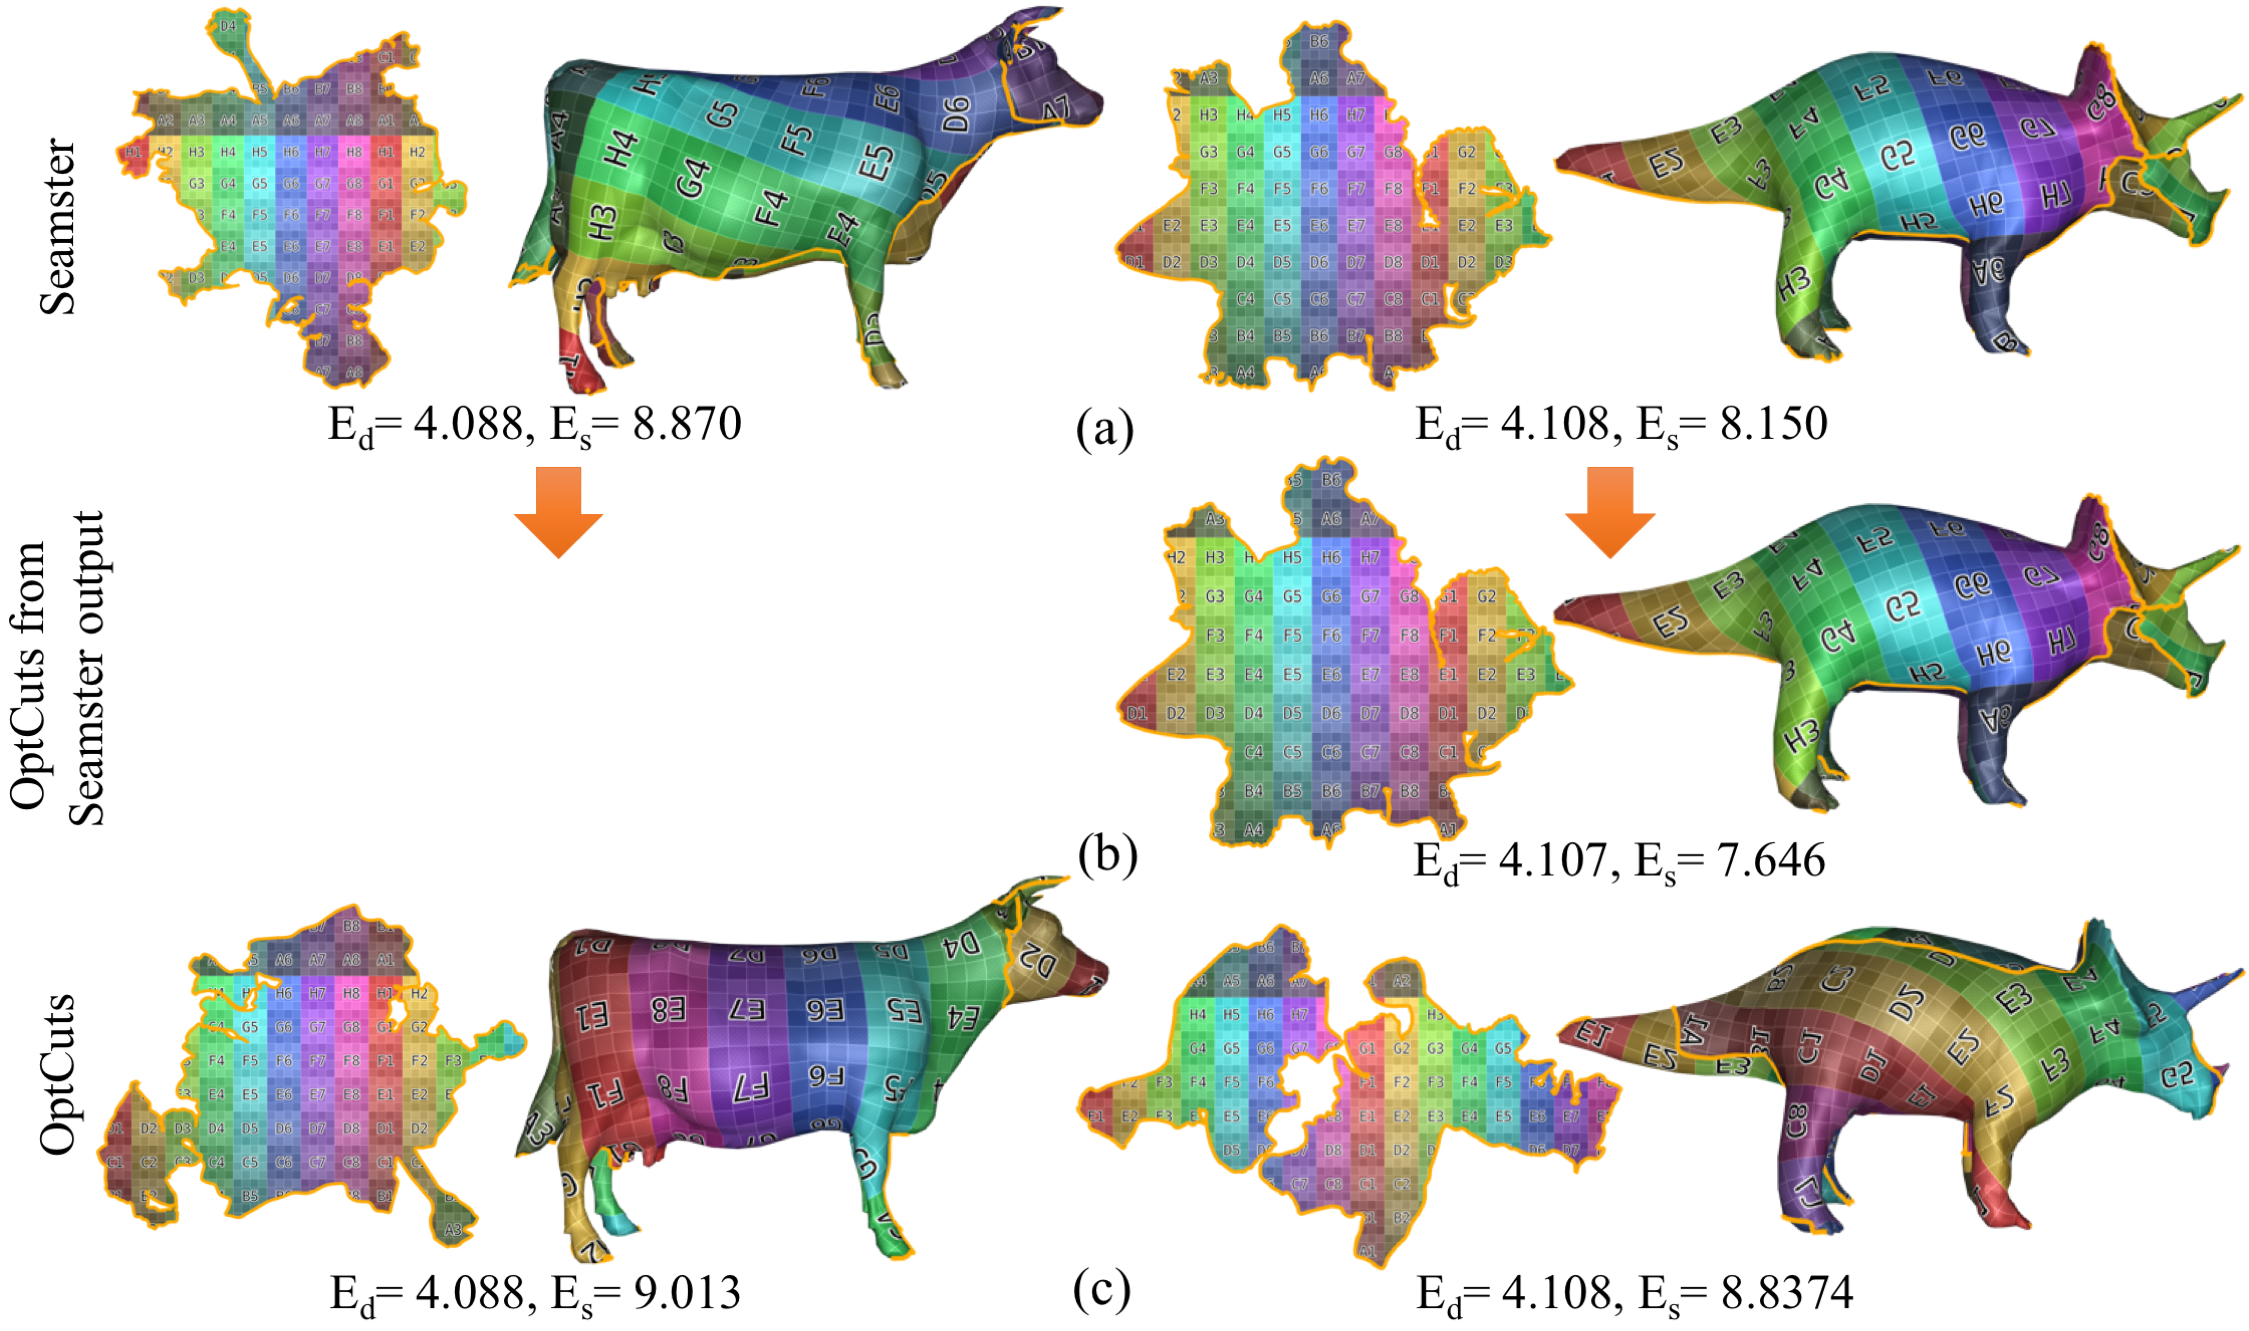
\includegraphics[width=\linewidth]{fig/comp_Seamster.png}
\caption{Comparison between Seamster and our method with bijectivity.}
\label{fig:comp_Seamster}
\end{figure}

\subsection{Variations}

Without changing the framework, simply reformulating $L = E_s + \lambda E_d$ according to different needs enables OptCuts to solve mesh parameterization problems in many variations:

\paragraph{Regional Seam Placement}
In texture painting applications, users would really like regions with the same semantic meanings stay connected or close to each other on the UV map. If we let users to select those regions on the input surface, we could easily avoid seams in those regions while still achieving bijectivity and similar seam length under the same distortion bound (Figure~\ref{fig:regional_seam_placement}). The only modification to our formulation is to reweight $E_{SL}$ with the indicator function provided by the user as
\[ E_s = \hat{E}_{SL} = \sum_{i\in\mathcal{S}} w_{SL,i} E_{SL,i} \quad w_{SL,i} \in [1.0, +\infty] \]

\begin{figure}[!h]
\centering
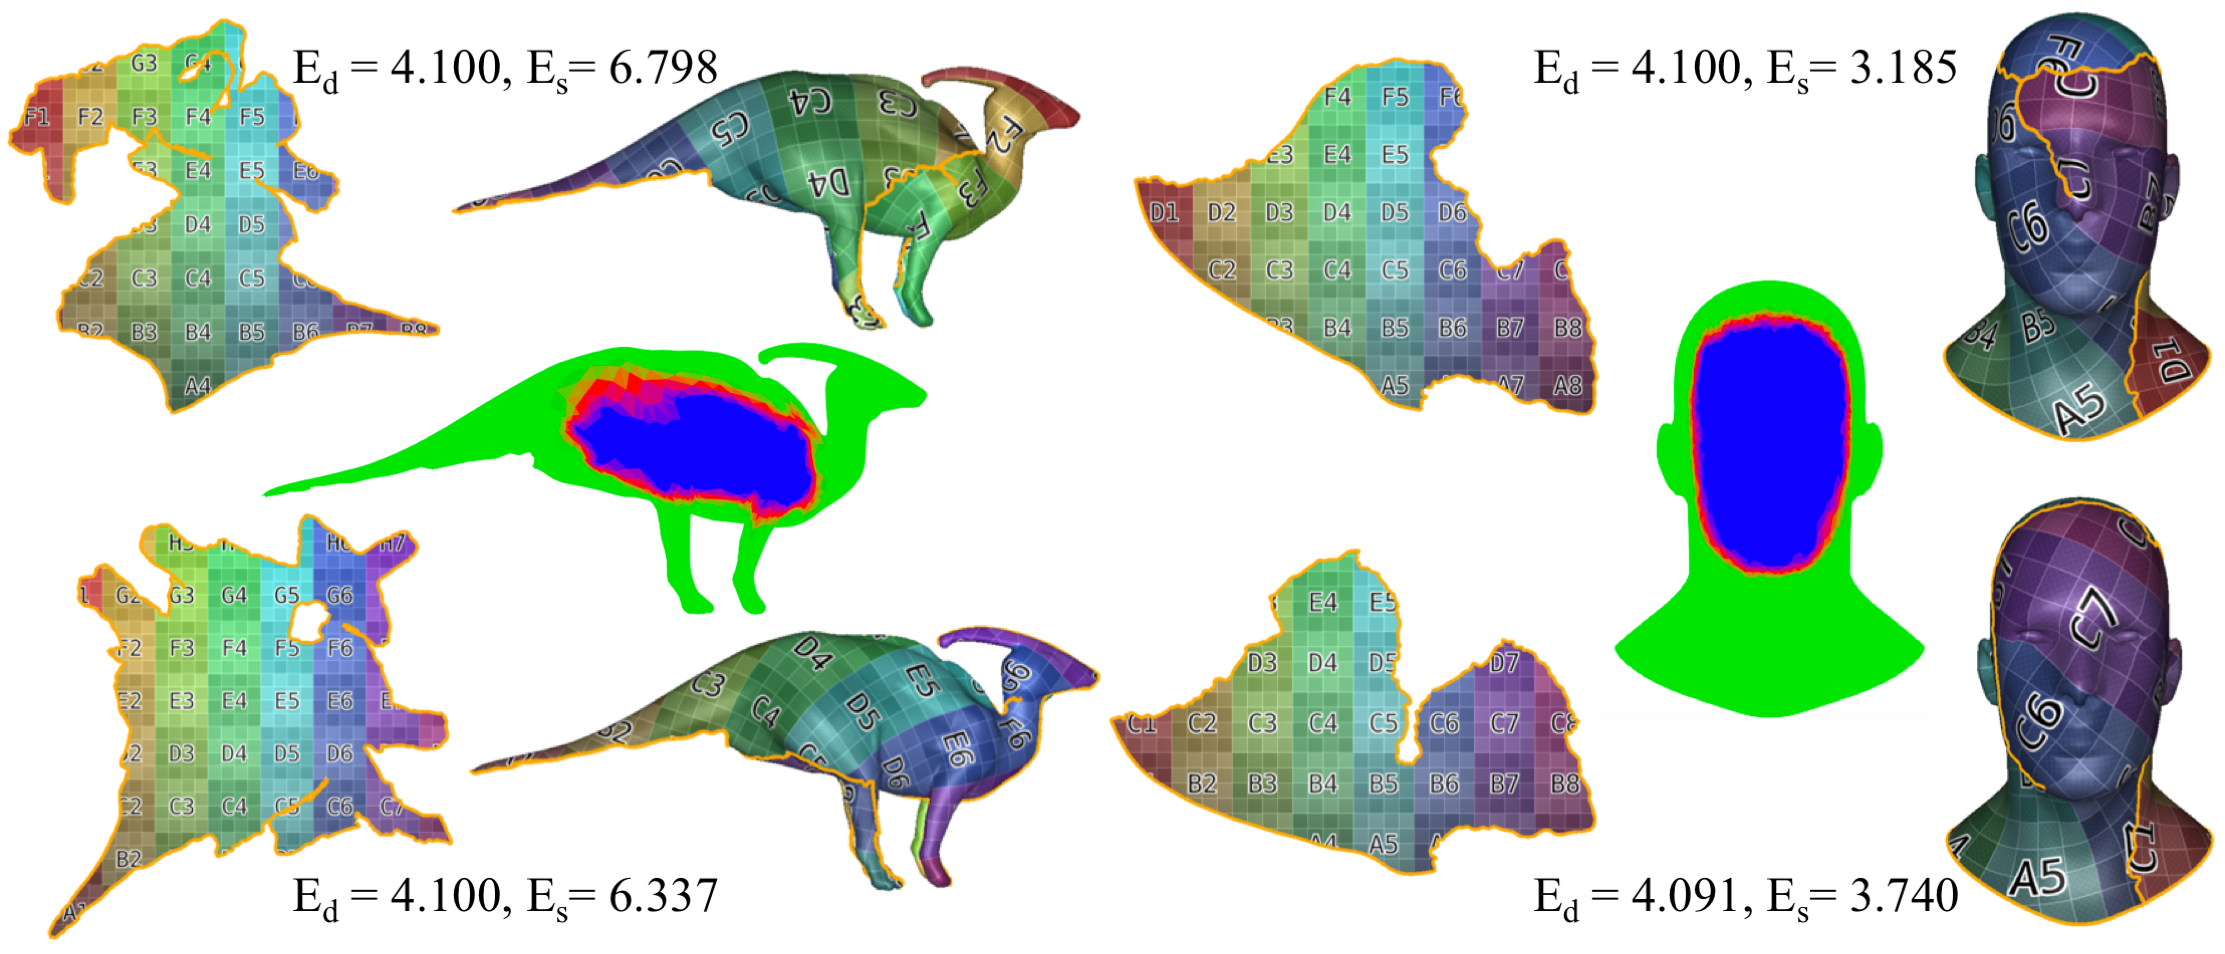
\includegraphics[width=\linewidth]{fig/regional_user.png}
\caption{Two examples of user controlled regional seam placement. Up to bottom: UV maps generated by the standard version of our method with bijectivity and $b_d = 4.1$, user preference on regional seam placement (blue means seams are less wanted), UV maps generated by the variation of our method supporting the given user preference (with bijectivity and $b_d = 4.1$).}
\label{fig:regional_seam_placement}
\end{figure}

\paragraph{Conformal Parameterization}
\minchen{[do we want this?]}
Using a conformal energy~\cite{Hormann2000MIPS,Sheffer2005ABFPP} for $E_d$ will achieve joint seam placement and conformal parameterization. Figure~\ref{fig:conformal_vs_isometry} shows some results with $E_d = E_{ABForMIPS}$~\cite{} compared to results with $E_d = E_{SD}$, where different seams are generated while our framework stays the same.

\paragraph{Different Cutting Strategy}
\minchen{[do we want this?]}
Geometry Images iteratively finds an extremal point with maximal $L^2$ stretch~\cite{} on the current UV map and make a cut, connecting the extremal point to the current seam with shortest path on the input surface, to reduce distortion on the newly parameterized map. To fairly compare with Geometry Images' cutting strategy, instead of using shape preserving mesh parameterization~\cite{} to always generate a circled UV map, we here change it by minimizing the symmetric Dirichlet energy for parameterization between each cut. Now that our Geometry Images is based on a free-boundary parameterization, the distortion will always decrease after a new cut is introduced, thus we can also set a distortion bound to terminate the algorithm when the bound is reached.

Given the same input surface with our standard UV initialization, we reach identical distortion bounds with shorter seam length (Figure~\ref{fig:comp_GI}). Note that when we asked for more and more isometric UV maps, the quality of the seams by Geometry Images drop drastically while our method keeps generating high-quality seams (See batch comparison statistics in Table~\ref{tb:comp_GI}).

\begin{figure}[!h]
\centering
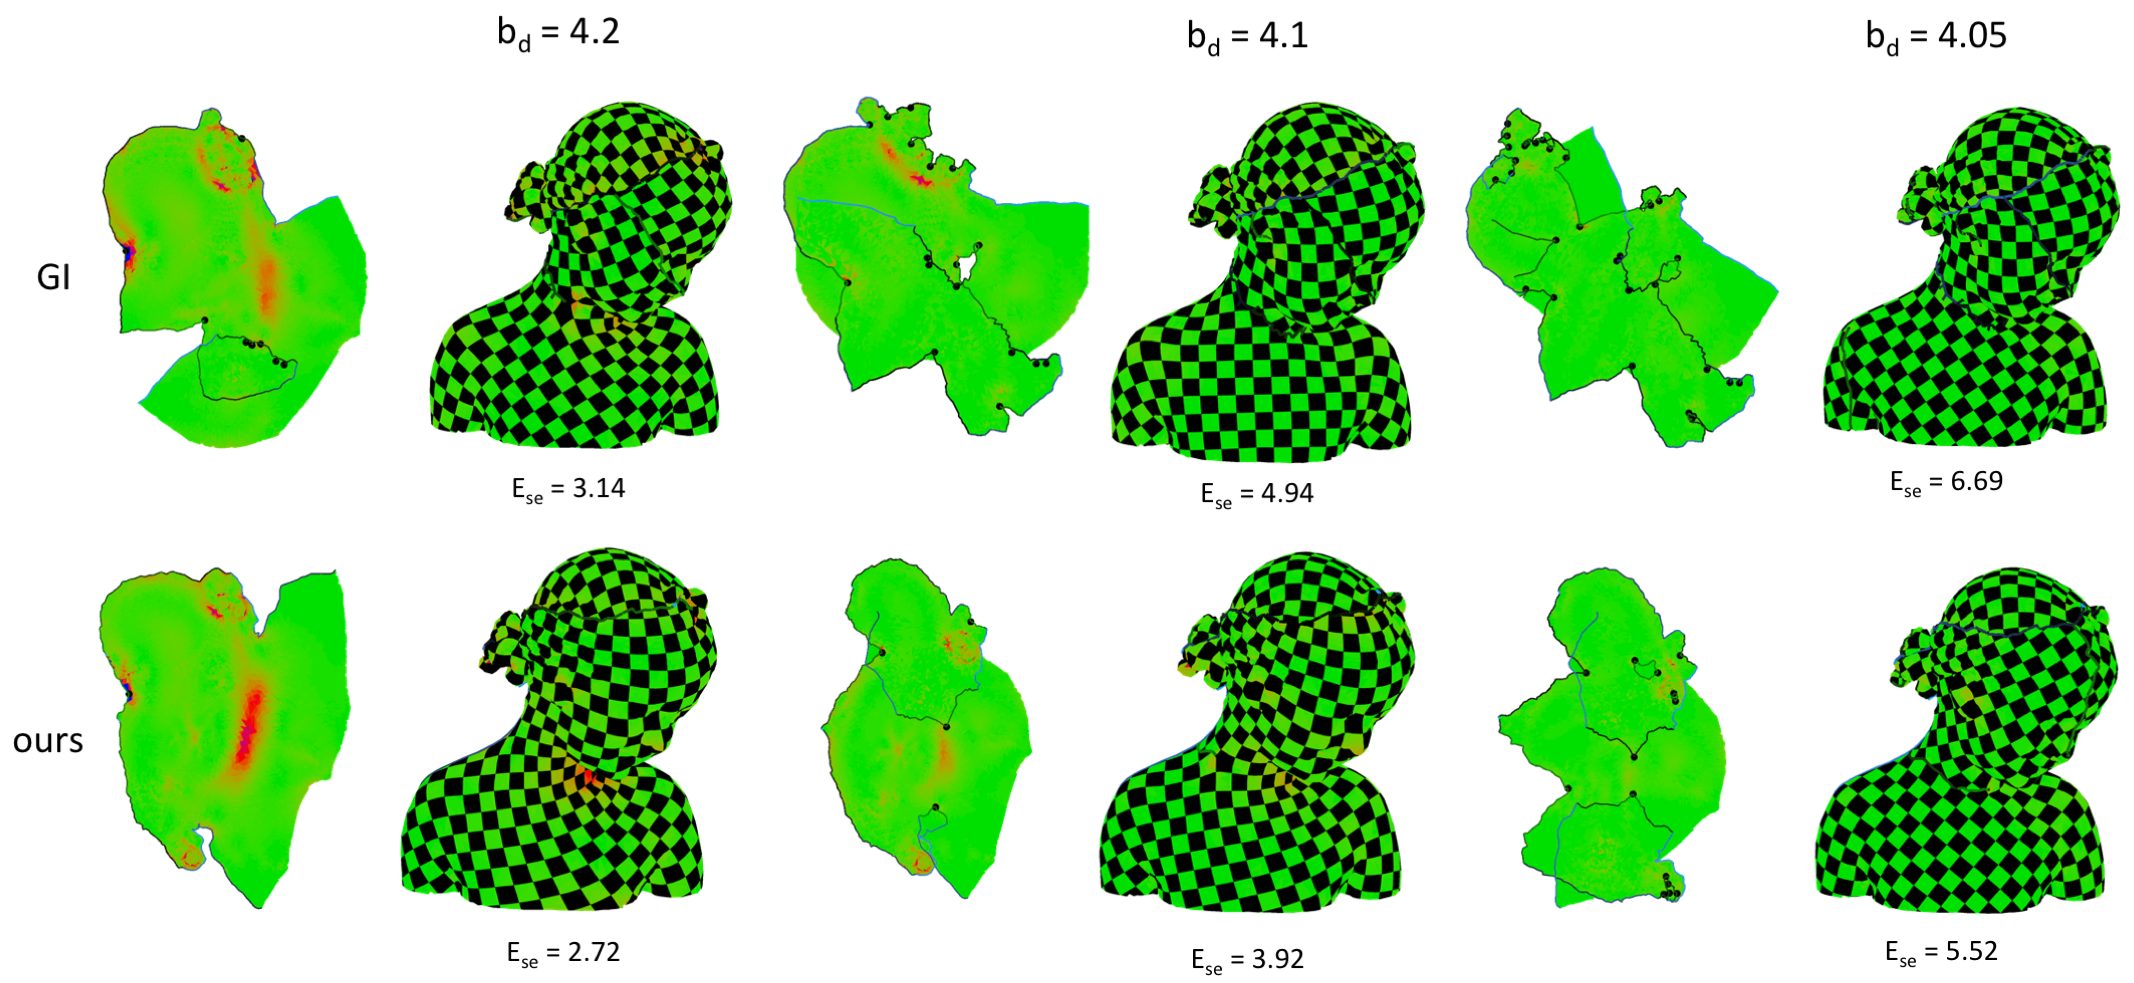
\includegraphics[width=\linewidth]{fig/comp_GI.png}
\caption{Comparison between Geometry Images and our method on the bimba model with $b_d = 4.2, 4.1, 4.05$ from left to right.}
\label{fig:comp_GI}
\end{figure}
% also could be face_f10000, male_body_i_f10000, statue_3_i_f10000, statue_4_i_f10000, statue_5_i_f10000

\begin{table}[!h]
\centering
\caption{Comparisons between Geometry Images and our method on 70 input surfaces with $3721$ vertices per input in average. Two $E_{SL}$ are considered to be similar if their ratio lies inside $[0.95, 1.05]$.\minchen{Percentage when our $E_{SL}$ is smaller is 58.9\%, 60.3\%, and 64.0\% for $b_d = 4.2, 4.1, 4.05$. Which kind of stats is stronger?} In the last row we start our optimization from the output seams by GI with $b_d = 4.1$ and generates bijective UV maps.} 
\label{tb:comp_GI}
\begin{tabular}{@{}cccccccc@{}}
\toprule
\multirow{2}{*}{$b_d$} & \multicolumn{2}{c}{average $E_{SL}$}             & \multicolumn{3}{c}{when our $E_{SL}$ is}                         & \multicolumn{2}{c}{average time (s)}       \\ \cmidrule(l){2-8} 
                   & GI & ours & shorter & similar & longer & GI & ours \\ \midrule
4.2                & 4.03             & 3.98           &  47.9\%  & 17.8\%  & 34.2\% & 13.0          & 87.0        \\
4.1                & 4.93             & 4.84           &  43.8\%  & 30.1\%  & 26.0\% & 17.0        & 137.5        \\
4.05               & 6.33             & 6.14           &  45.3\%  & 36.0\%  & 18.7\% &  24.1        & 213.2        \\ 
4.1*               & 4.93             & 4.79           &  48.6\%  & 36.1\%  & 15.3\% &  17.0        & 304.0        \\ \bottomrule
\end{tabular}
\end{table}

If we take Geometry Images output as a fast heuristic initial guess, we can use OptCuts to improve the seam quality towards the locally optimal point while still satisfying the distortion bound. To make this experiment more challenging, we add bijectivity constraints to our framework, which prevents from reaching below the distortion bound with the initial seams. However, we still efficiently obtain bijective UV maps with even shorter seams (Figure~\ref{fig:comp_GI_outputAsInit}, Table~\ref{tb:comp_GI} last row).

\begin{figure}[!h]
\centering
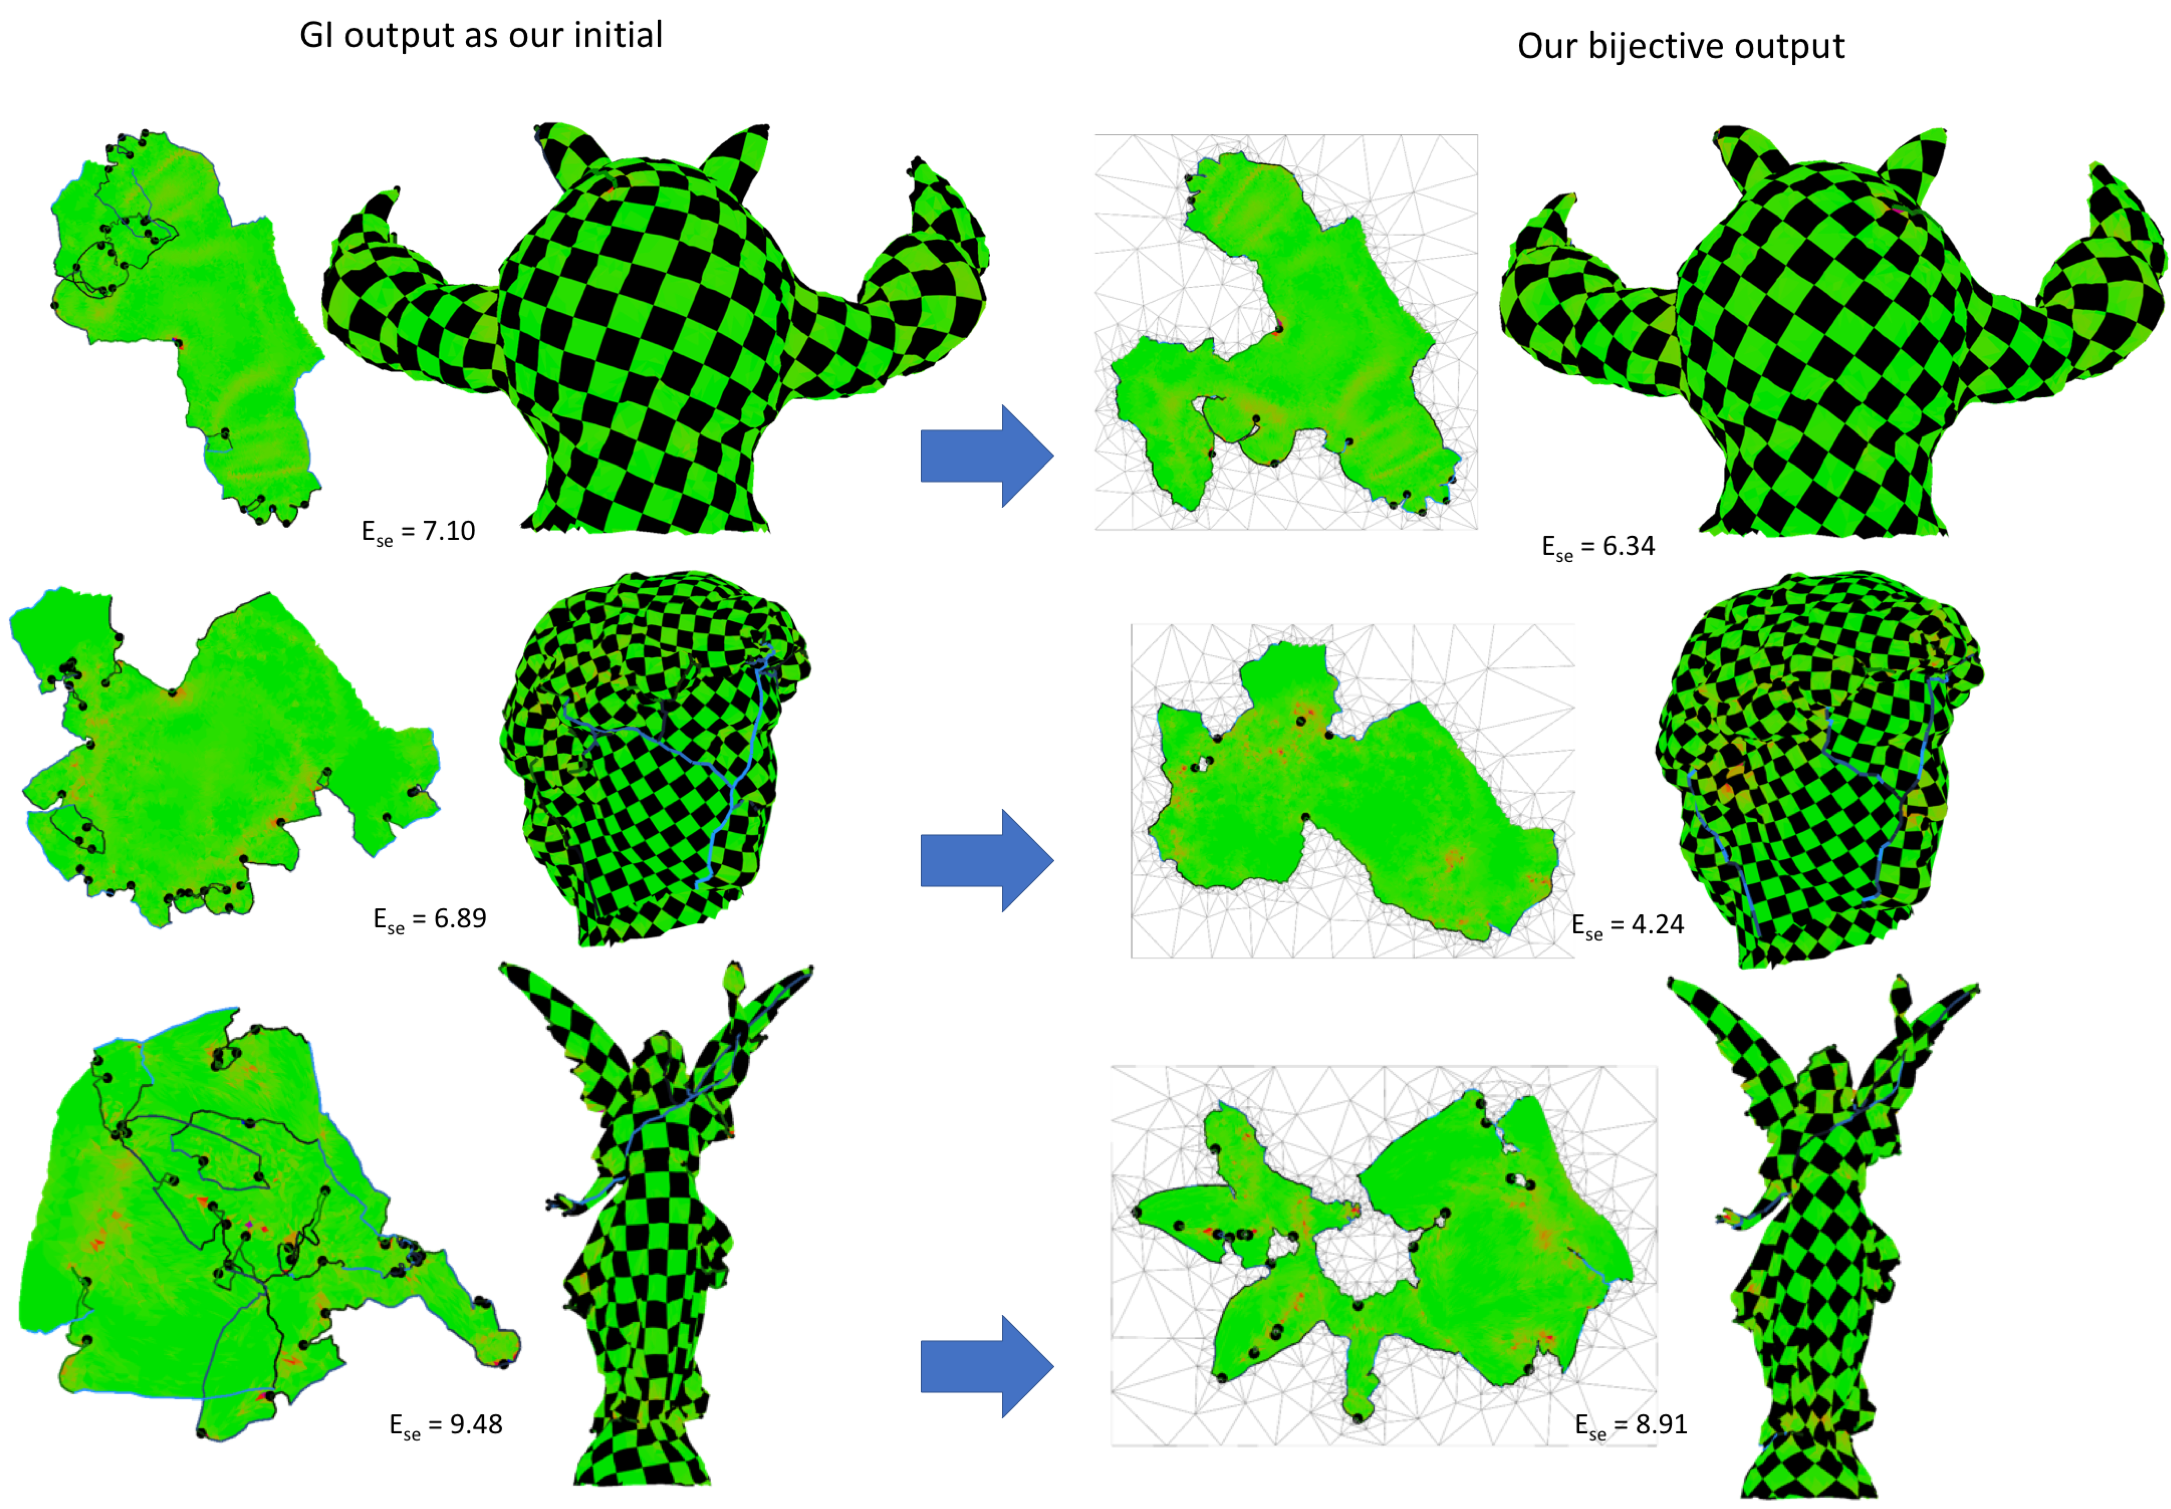
\includegraphics[width=\linewidth]{fig/comp_GI_outputAsInit.png}
\caption{Using Geometry Images output with $b_d = 4.1$ as our initial UV map and distortion bound, we improve seam quality, reaching a locally optimal seam configuration, even with an extra bijectivity constraints.}
\label{fig:comp_GI_outputAsInit}
\end{figure}
% also could be bimba, bunny

The key is that with all these variations, our framework stays the same, and it efficiently generates optimal seams for the specific problem formulation.
